
\section{Einleitung}
In diesem Versuch wird das Energiespektrum und verschiedene Absorptionssektren einer
Kupferröntgenröhre untersucht werden.
\section{Theorie}
Innerhalb einer evakuierten Röhre kann Röntgenstrahlung erzeugt werden. Aus einer Glühkathode
werden Elektronen emittiert und auf eine Anode beschleunigt. Durch das Aufreffen der beschleunigten
Elektronen auf die Anode entsteht Röntgenstrahlung, die aus einem kontinuerliches Bremsspektrum
und charakteristische Strahlung besteht.
\newline
Durch das Abbremsen eines Elektrons im Coulombfeld eines Atomkerns wird ein Photon ausgesendet.
Dabei eintspricht die Energie des Photons dem Energieverlust des abgebremsten Elektrons.
Für den Fall, dass die gesamte kinetische Energie in Strahlungsenergie umgewandelt wird, ist die Energie
maximal. Die minmiale Wellenlänge des kontinuerlichen Bremsspektrums wird durch
\begin{equation}
  \lambda_\text{min}=\frac{h\cdot c}{e_0U}
  \label{eqn:wellenlänge}
\end{equation}
beschrieben. Dabei ist U die Beschleunigungsspannung.
\newline
Durch die Ionisation des Anodenmaterials entsteht eine Leerstelle in einer inneren Schale.
Diese Leerstelle wird unter Aussendung eines Röntgenquants von einem Elektron aus einer äußeren Schale aufgefüllt.
Dabei entspricht die Energie des ausgesendeten Röntgenquants der Differenz des Energieniveaus
$h\nu =E_m-E_n$. Die Energie ist dabei charakteristisch für das Anodenmaterial der Röntgenröhre,
weshalb hier von einem charaktertistischen Spektrum gesprochen wird. Durch Abschirmungseffekte der
Hüllenelektronen und der Wechselwirkungen der Elektronen untereinander, verringert sich die Bindungsenergie
eines äußeren Elektrons. Für diese Bindungsenergie gilt
\begin{equation}
  E_n=-R_\text{ryd} z_\text{eff}^2\frac{1}{n^2}.
  \label{eqn:bindungsenergie}
\end{equation}
Dabei ist die effektive Kernladung $z_\text{eff}=z-\sigma$, wobei $\sigma$ die Abschirmkonstante ist und $R_\text{ryd}$ die
Rydbergenegie. Zu jedem Elektron können aufgrund unterschiedlicher Bindungsenergien charaktertistische
Linien zugeordnet werden. Diese werden als Feinstruktur bezeichnet.
\newline
Für diesen Versuch werden allerdings nur $\symup{K}_\alpha$- und $\symup{K}_\beta$ Kupferlinien betrachtet.
Der Comptoneffekt und der Photoeffekt sind für die Absorption von Röntgenstrahlung unter $\SI{1}{MeV}$
die dominanten Absorptionsprozesse. Die Absorption nimmt mit zunehmender Energie ab und steigt sprunghaft wieder an,
wenn die Photonenenergie größer ist als die Bindungsenegerie eines Elektrons aus der nächsten tieferen Schale.
Die Abschirmkonstante lässt sich durch
\begin{equation}
\sigma_L=Z-\biggl(\frac{4}{\alpha}\sqrt{\frac{\Delta E_L}{R_\text{ryd}}}-\frac{5\Delta E_L}{R_\text{ryd}}\biggr)^\text{1/2}\biggl(1+\frac{19}{32}\alpha^2\frac{\Delta E_L}{R_\text{ryd}}\biggr)^\text{1/2}.
\label{eqn:sigma}
\end{equation}
berechnen.
Hierbei ist $\Delta E_L$ die Energeidifferenz zwischen $E_{L_\text{II}}$- und $E_{L_\text{III}}$-Absorptionskante,
Z die Ordungszahl und $\alpha$ die Feinstrukturkonstante.
\newline
Mithilfe von dreidimensionalen Gittern kann experimentell die Wellenlänge und somit auch die Energie
der Röntgenstrahlen ermittelt werden. Unter der Bragg'schen Reflexion werden Photonen an jedem Atom
der Gitters gebeugt. In dem Glanzwinkel $\theta$ kommt es zur konstrukttiven Interferenz der Wellenlängen.
Die Bragg-Bedingung formuliert die folgende Abhängigkeit zwischen der Gitterkonstante d, der gebeugten Wellenlänge $\lambda$
und der Beugungsordnung n:
\begin{equation}
2d\sin(\theta)=n\lambda.
\label{eqn:bragg}
\end{equation}
\section{Durchführung}
%Der Versuchsaufbau ist in Abbildung \ref{fig:aufbau} zu sehen.
%\begin{figure}
%  \centering
%  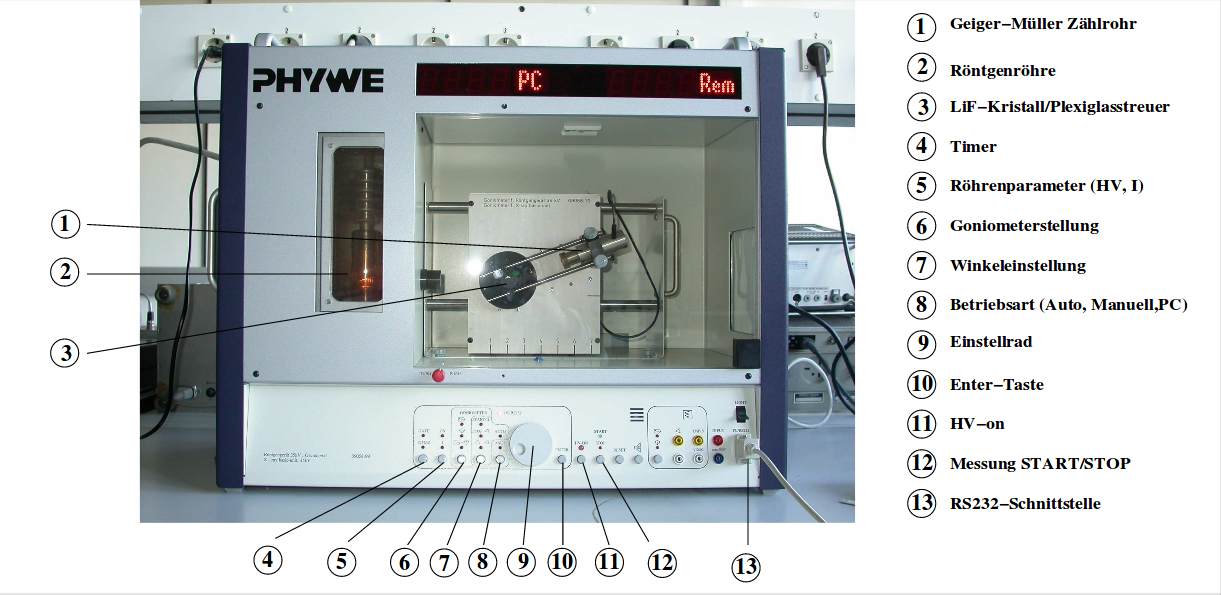
\includegraphics[scale=0.40]{aufbau.png}
%  \caption{Aufbau zur Untersuchung der Emission und Absorption einer Röntgenröhre.\cite{anleitung}}
%  \label{fig:aufbau}
%\end{figure}
%\newline
Für diesen Versuch wird eine Kupfer-Röntgenröhre, ein LiF-Kristall und ein Geiger-Müller-
Zählrohr verwendet. Bei allen Messungen wird eine Beschleunigerspannung von $\SI{35}{kV}$ und
ein Strom von $\SI{1}{\milli\ampere}$ verwendet.


Zu erst wird die Bragg-Bedingung überprüft. Dafür wird ein Glanzwinkel von $\Theta = 14°$ eingestellt.
Bei einer Winkeländerung von $\Delta\alpha_{GM} = 0,1°$ wird in einem Winkelbereich des Geiger-Müller-Zählrohrs
von $\alpha_{GM} = 26°$ bis $30°$ die Intensität der Röntgenstrahlung gemessen.
\newline
Als nächstes wird das Eimssionsspektrum einer Kupfer-Röntgenröhre bestimmt. Dabei wird wieder das
Messgerät in den 2:1 Koppelmodus gestellt und in $\Theta = 0.2°$-Schritten die Winkel zwischen $\Theta = 4°$ bis $26°$
gemessen. Die Integrationszeit jedes Winkels beträgt dabei $\Delta{t} = 5$\,s.


Zum Schluss wird das Absorptionsspektrum von mehrern Absorbern bestimmt. Die Proben Brom, Strontium und Zirkonium
werden für die Elemente mit einer Ordungszahl zwischen $ 30 \leq Z \leq 50$ und Quecksilber für das Element mit einer
Ordungszahl $Z \geq 70$ ausgewählt.
